\documentclass{article}
\usepackage[UTF8]{ctex}
\setmainfont{Calibri Light}
\usepackage{setspace}
\renewcommand{\baselinestretch}{1.2}
\usepackage{amsmath,bm}
\usepackage{framed} 
\usepackage{wrapfig}
\usepackage{amssymb}
\usepackage{ntheorem}
\usepackage{graphicx}
\usepackage{bbm}
\usepackage{hyperref}
\hypersetup{
	colorlinks=true,
	linkcolor=blue,
	filecolor=cyan,      
	urlcolor=red,
	citecolor=green,
}
\newtheorem{theorem}{Theorem}
\newtheorem{corollary}{Corollary}
\newtheorem{lemma}{Lemma}
\newtheorem*{proof}{Proof}
\setlength{\parindent}{2em}
\author{Siheng Zhang\\zhangsiheng@cvte.com}
\title{Chapter \textbf{\textit{4}} Linear Model}
\date{\today}
\usepackage[a4paper,left=18mm,right=18mm,top=25mm,bottom=25mm]{geometry} 

\begin{document}
\maketitle  

This part corresponds to \textbf{Chapter 1,3,4 of PRML, Chapter of UML}, and mainly answers the following questions:

\begin{itemize}
\item 
\end{itemize}

\tableofcontents
\newpage

\section{Linear classification}

	In the last chapter, we stops at the linear classification of binary classification task,
	
	\begin{equation}
	h(\mathbf{x})=\mathbf{w}^\top \mathbf{x} + w_0 = \sum_{j=1}^d w_j x_j + w_0
	\label{eq:linear}
	\end{equation}
in which $\mathbf{w}$ is weight vector, and $w_0$ is bias. The input vector is assigned to class $C_1$ iff. $h(\mathbf{x})\geq 0$ and to class $C_2$ otherwise.

	Consider two points $\mathbf{x}_1,\mathbf{x}_2$ on the decision boundary, i.e., $\mathbf{w}^\top (\mathbf{x}_1 - \mathbf{x}_2) = 0$, hence $\mathbf{w}$ is orthogonal to the decision boundary. And the distance from the origin to the decision boundary is $\mathbf{w}^\top \mathbf{x} / \|\mathbf{w}\|=-w_0/\|\mathbf{w}\|$.
	
	\begin{framed}
	\begin{scriptsize}
	\begin{spacing}{1.2}
	\noindent\textit{\textbf{remark1.} For convenience, we introduce an additional input value $x_0 = 1$ and define $\tilde{\mathbf{w}} = (w_0, \mathbf{w})$ and $\tilde{\mathbf{x}} = (x_0, \mathbf{x})$ so that $h(\mathbf{x}) = \tilde{\mathbf{w}}^\top \tilde{\mathbf{x}}$. We neglect the `tilde' symbol below.}
	
	\noindent\textit{\textbf{remark2: extend to multiple classes.}  \textbf{one-versus-the-rest} For each class $k=1,2,...,K$, each classifier judge whether an example is $C_k$ or not. So there are $K$ classifiers needed;  \textbf{one-versus-one} An alternative is to introduce $\frac{K(K-1)}{2}$ binary discriminant functions, one for every pair of classes (but will lead to ambiguous region).}
	\end{spacing}
	\end{scriptsize}
	\end{framed}
	
	\subsection{The VC dimension of half-spaces}
	
	The class of linear function (Eq. \ref{eq:linear}) represents a hypothesis set  \textit{half-space}, usually denoted as $HS_d$. Its VC dimension is $VCdim(HS_d)=d+1$.  It follows that we can learn half-space using the ERM paradigm with a sample size of $\Omega(\frac{d+\log(1/\delta)}{\epsilon})$. 

	\begin{framed}
	\begin{scriptsize}
	\begin{spacing}{1.2}
	\noindent\textit{\textbf{remark3: proof.} Firstly, we should show that any set of $d+1$ points in $\mathcal{R}^d$ can be shattered by $HS_d$. Consider the set of vectors $\mathbf{0}, \mathbf{e}_1, ..., \mathbf{e}_d$ where for every i the vector $\mathbf{e}_i$ is the all zeros vector except 1 in the i-th entry. This set can be shattered by $HS_d$ by set $\mathbf{w}=[y_1-b,\cdots,y_d-b,b]$.}
	
	\textit{Secondly, we should show there exists a point set of $d+2$ points in $\mathcal{R}^{d}$ that cannot be shattered by half-space. Denote the points as $\mathbf{x}_1, \mathbf{x}_2, \cdots, \mathbf{x}_{d+1}, \mathbf{x}_{d+2}$. There must be some $a_i, i=1,2,\cdots,d+2$ (not all of them are zero) which satisfy that $\sum_{i=1}^{d+2} a_i \mathbf{x}_i = \mathbf{0}$. Split the $a_i$ into two sets $I={i,a_i>0}$ and $J={i,a_i<0}$, then we have }
	
	\begin{equation*}
	\sum_{i\in I} a_i \mathbf{x}_i = \sum_{i \in J} |a_i| \mathbf{x}_i
	\end{equation*}
	\textit{If the VC dimension is $d+1$, then there must be some $\mathbf{w}$ such that $\mathbf{w}^\top \mathbf{x}_i > 0, \forall i \in I$ and $\mathbf{w}^\top \mathbf{x}_i < 0, \forall i \in J$. It follows that}
	
	\begin{equation*}
	0 < \sum_{i \in I} a_i \mathbf{w}^\top \mathbf{x}_i = \mathbf{w}^\top  \sum_{i \in I} a_i \mathbf{x}_i = \mathbf{w}^\top  \sum_{i \in J} |a_i| \mathbf{x}_i =  \sum_{i \in J} |a_i| \mathbf{w}^\top \mathbf{x}_i  < 0
	\end{equation*}
	\noindent\textit{which leads to a contradiction.}
	\end{spacing}
	\end{scriptsize}
	\end{framed}
	
	\subsection{Solution}
	
	\begin{itemize}
	\item \textbf{linear programming (LP) solver for realizable case.} In the realizable (namely, separable) case, we can implement ERM paradigm as a linear programming problem with dummy objective. LP has the common form of
	\begin{equation*}
	\begin{split}
	&\min_\mathbf{w} \mathbf{u}^\top \mathbf{w} \\
	s.t. & \mathbf{Aw} \geq \mathbf{v}
	\end{split}
	\end{equation*}
	
	Since we are looking for $\text{sign}(\mathbf{w}^\top \mathbf{x}_i)=y_i$, i.e., $y_i(\mathbf{w}^\top \mathbf{x}_i)> 0, \forall i$. Define $\gamma=\min_i y_i(\mathbf{w}^\top \mathbf{x}_i)$ and let $\mathbf{w}'=\frac{\mathbf{w}}{\gamma}$, then we have $y_i(\mathbf{w}'^\top \mathbf{x}_i)\geq 1 $. With a dummy objective, it leads to LP's form.
	
	\item \textbf{least-squares solution.} Least squares is the algorithm that implements the ERM rule for the hypothesis class with respect to the squared loss. The weight vector can be determined by minimizing a sum-of-squares error function $\sum_i \|\mathbf{y}_i-h(\mathbf{x}_i)\|^2$. Setting the derivative w.r.t. weight to be zero leads to $\mathbf{w} = \mathbf{X}^\dagger \mathbf{Y} = (\mathbf{X}^\top \mathbf{X})^{-1} \mathbf{X}^\top \mathbf{Y}$, in which $\mathbf{X}\in \mathcal{R}^{n\times d}$, each row is $\mathbf{x}^\top$. $\mathbf{X}^\dagger$ is the  \textit{Moore-Penrose pseudo-inverse} of $\mathbf{X}$.
	
	Linear classification treats a problem with multiple targets to be multiple problems with single target each problem. If every target vector satisfies some  linear constraint $\mathbf{a}^\top \mathbf{y} + b = 0$, then the model prediction given by least-squares solution is $\mathbf{a}^\top h(\mathbf{x}) + b = 0$. Thus if we use a one-hot encoding for $K$ classes, the predictions made by the model will sum up to 1. However, this constraints alone is not sufficient to allow the model outputs to be interpreted as probability because they may not lie in the interval $(0,1)$.

	\item \textbf{perceptron algorithm.} Besides, we can also use a perceptron algorithm to implement ERM rule, which is left in the next chapter.	
	\item \textbf{surrogate loss.} In the agnostic (namely, non-separable) case, the implementation is computational hard. The most popular solution is to use surrogate loss functions but not the 0-1 loss in realizable case, which is left in \ref{sec-lr}.
	
	\end{itemize}
	
	\subsection{Fisher's linear discriminant}
	
	One way to view a linear classification model is in terms of \textit{dimensionality reduction}, \textit{i.e.}, projection from $\mathcal{R}^d$ to $\mathcal{R}$. By adjusting the components of the weight vector $\mathbf{w}$, we can select a projection that maximizes the class separation. To begin with, consider a two-class problem ($N_1$ points of class $C_1$ and $N_2$ points of class $C_2$), so that the mean vectors of the two classes are given by $\mathbf{m}_k = \frac{1}{N_k} \sum_{\mathbf{x}_n \in C_k} \mathbf{x}_n, k=1,2$.

	The simplest measure of the separation of the classes, when projected onto $\mathbf{w}$, is the separation of the projected class means. This suggests that we might choose $w$ so as to
	\begin{equation*}
	\max_\mathbf{w} m_2- m_1=\mathbf{w}^\top (\mathbf{m}_2-\mathbf{m}_1)
	\end{equation*}
where $m_k=\mathbf{w}^\top \mathbf{m}_k$ is the mean of the projected data from class $C_k$. 

	This expression can be made arbitrarily large simply by increasing the magnitude of $\mathbf{w}$. To solve this problem, we could constrain $\mathbf{w}$ to have unit length, i.e., $\|\mathbf{w}\|_2=1$. Using a Lagrange multiplier, it turns to maximize $\mathbf{w}^\top (\mathbf{m}_2-\mathbf{m}_1) + \lambda (\|\mathbf{w}\|_2-1)$, which leads to $\mathbf{w}\propto \mathbf{m}_2-\mathbf{m}_1$.
	
	\begin{wrapfigure}{r}{10cm}
	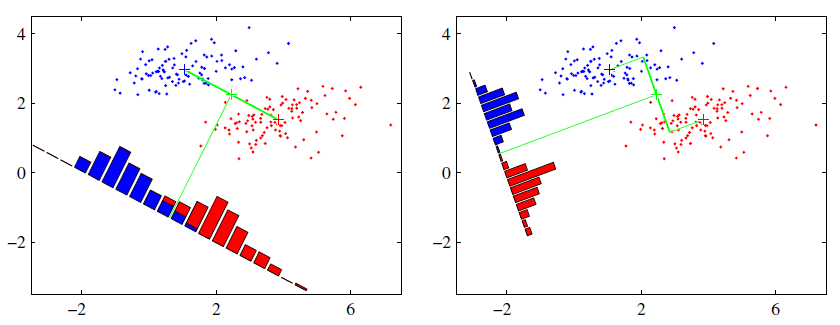
\includegraphics[scale=.7]{C4 fisher.png}	
	\label{fig4.1}
	\end{wrapfigure}
However, some outliers, which lays far from its class and close to the other class, may be mis-classified after projection, even though the dataset is linearly separable (see figure \ref{fig4.1}). This indicates that the objective above still needs to be improved. In fact, besides maximizing the separation margin, the projection is expected to reduce the inner-class variance. Denote the variance as $s_k^2=\sum_{\mathbf{x}_n\in C_k} (\mathbf{w}^\top\mathbf{x}_n-m_k)^2$, the objective is given by
	
	
	\begin{equation}
	\max_\mathbf{w} J(\mathbf{w}) = \frac{(m_2-m_1)^2}{s_1^2+s_2^2} 
	= \frac{\mathbf{w}^\top \mathbf{S}_B \mathbf{w}}{\mathbf{w}^\top \mathbf{S}_W \mathbf{w}}
	\end{equation}
in which $\mathbf{S}_B=(\mathbf{m}_2-\mathbf{m}_1)(\mathbf{m}_2-\mathbf{m}_1)^\top, \mathbf{S}_W=\sum_{k=1}^2\sum_{\mathbf{x}_n\in C_k}(\mathbf{x}_n-\mathbf{m}_k)(\mathbf{x}_n-\mathbf{m}_k)^\top$. Setting the derivative to zero leads to $(\mathbf{w}^\top \mathbf{S}_B \mathbf{w}) \mathbf{S}_W \mathbf{w} = (\mathbf{w}^\top \mathbf{S}_W \mathbf{w}) \mathbf{S}_B \mathbf{w}$. Since we just need the direction, we can neglect scalar factors. Besides,  $\mathbf{S}_B \mathbf{w}$ is always in the direction of $\mathbf{m}_2 - \mathbf{m}_1$. So the optimizer is $\mathbf{w}\propto \mathbf{S}_W^{-1} (\mathbf{m}_2-\mathbf{m}_1)$.
	
	\begin{framed}
	\begin{scriptsize}
	\begin{spacing}{1.2}
	\noindent\textit{\textbf{remark6: Isotropic.} If $\mathbf{S}_W$ is unit matrix (i.e., the data distribution of each class is isotropic), then the solution degenerates to $	\mathbf{w}\propto \mathbf{m}_2-\mathbf{m}_1$.} 
	
	\noindent\textit{\textbf{remark7: Fisher's linear discriminant for the case of multi-class.}}
	\end{spacing}
	\end{scriptsize}
	\end{framed}
		
	\subsection{Probabilistic perspective}
	
	\subsubsection{Logistic regression}
	\label{sec-lr}
	
	\subsubsection{Iterative re-weighted least squares(IRLS)}

\section{Linear regression}

	In linear regression model, the model is the same except that the learning target $y$ is continuous but not discrete. And the learning goal is the sum-of-square (SSE) loss

	\begin{equation}
	\min_\mathbf{w} L_S(h) =\sum_{i=1}^m  l(h(\mathbf{x}_i)) = \sum_{i=1}^m (h(\mathbf{x}_i) - y_i)^2 = \sum_{i=1}^m (\mathbf{w}^\top\mathbf{x}_i - y_i)^2 
	\end{equation}

	Suppose the fitting error $\epsilon_i = y_i-\mathbf{wx}_i$ is Gaussian noise, i.e., $\epsilon_i \sim\mathcal{N}(0,\beta)$. Then the log likelihood function of the training sequence is
	
	\begin{equation*}
	\log \mathcal{L} = -\frac{m}{2} \log 2\pi\beta - \sum_{i=1}^m \frac{(y_i-\mathbf{w}^\top\mathbf{x}_i)^2}{2\beta}
	\end{equation*}
Obviously, MLE is equivalent to linear regression.

	\begin{framed}
	\begin{scriptsize}
	\begin{spacing}{1.2}
	\noindent\textit{\textbf{remark8.} Since linear regression is not a binary prediction task, we cannot analyse its sample complexity using the VC-dimension. One possible analysis of the sample complexity of linear regression is by relying on the "discretization trick". However, to apply the sample complexity bounds from Chapter 2 we also need that the loss function will be bounded.}
	\end{spacing}
	\end{scriptsize}
	\end{framed}
	
	\subsection{Generalized linear regression}
	
	The model is just a linear function of the input variables, and this imposes significant limitations on it. Therefore, extended model considers \textbf{linear} combination of fixed \textbf{non-linear} functions of the input variables, of the form
	
	\begin{equation}
	h(\mathbf{x}) = w_0 + \sum_{j=1}^d w_j \phi_j(x)
	\end{equation}
where $\phi_j(x)$ are known as \textit{basis functions}. Again, denote $\phi_0(\mathbf{x})=1$ so that $h(\mathbf{x}) = \tilde{\mathbf{w}}^\top \phi(\mathbf{x})$. For Simplification, we also neglect the `tilde' symbol from now on.

	Least squares also gives the result by $\mathbf{w} = \Phi^\dag \mathbf{y} = (\Phi^\top \Phi)^{-1} \Phi^\top \mathbf{y}$. $\Phi$ is an $n*d$ matrix, whose elements are given by $\Phi_{nj} = \phi_j(\mathbf{x}_n)$.

	\begin{framed}
	\begin{scriptsize}
	\begin{spacing}{1.2}
	\noindent\textit{\textbf{remark9: multiple-outputs.} The solution to multiple-outputs regression problem decouples between the different target variables so we do not need to discuss it here.}
	
	\noindent\textit{\textbf{remark10: on-line learning.} Batch techniques involve processing the entire training set in one go, can be computationally costly for large data sets. For linear regression, stochastic gradient descent algorithm updates parameter using $\mathbf{w}^{t+1}=\mathbf{w}^{t} - lr*\nabla L_{(\mathbf{x}_t,y_t)}(h) = \mathbf{w}^{t} + lr* (y_i - (\mathbf{w}^t)^\top \mathbf{\phi} (\mathbf{x}_t)) \mathbf{\phi} (\mathbf{x}_t)$, in which $lr$ is the learning rate.}

	\noindent\textit{\textbf{remark11: Basis function examples.}} 1. \textbf{Polynomial basis}, 2. \textbf{Radical basis}, 3. \textbf{Fourier basis}.
	
	\end{spacing}
	\end{scriptsize}
	\end{framed}
	
	\subsection{Regularization \textit{a.k.a} Bayesian linear regression}
	
	In closed-form solution, if $n\leq d$, the SSE loss can achieve zero. It means that the model is able to 'memorize' all training examples, but the parameters vary significantly if the data points changes (even just a bit). So if there exists noisy data point, the model fits the noise well (zero training error) and will show bad performance to unseen data. This phenomenon is called \textbf{over-fitting}. Formally, consider the expected loss with squared error,
	\begin{equation*}
	\begin{split}
	\mathbb{E}(l) &= \int \int l(h(\mathbf{x})) p(\mathbf{x}, y) \text{d} \mathbf{x} \text{d}y \\
	&= \int \int (h(\mathbf{x})-y)^2 p(\mathbf{x}, y) \text{d} \mathbf{x} \text{d}y
	\ \ \ \ \footnotesize{\text{Note that, setting its derivatives to zero leads to $h(\mathbf{x}) = \int yp(\mathbf{x}, y) \text{d} y /p(\mathbf{x}) = \mathbb{E}(y|\mathbf{x})$}}\\
	&= \int \int \left\{ h(\mathbf{x}) - \mathbb{E} (y|\mathbf{x}) + \mathbb{E} (y|\mathbf{x}) - y \right\}^2 p(\mathbf{x}, y) \text{d} \mathbf{x} \text{d}y \\
	&= \int \left\{ h(\mathbf{x}) - \mathbb{E} (y|\mathbf{x}) \right\}^2 p(\mathbf{x}) \text{d} \mathbf{x} + \int \int \left\{\mathbb{E} (y|\mathbf{x}) - y \right\}^2 p(\mathbf{x}, y) \text{d} \mathbf{x} \text{d} y
	\end{split}
	\end{equation*}
	%&= \int \int \left\{ \left[ h(\mathbf{x}) - \mathbb{E} (y|\mathbf{x}) \right]^2 + \left[\mathbb{E} (y|\mathbf{x}) - y \right]^2 + 2 \left[ h(\mathbf{x}) - \mathbb{E} (y|\mathbf{x}) \right] \left[\mathbb{E} (y|\mathbf{x}) - y \right]  \right\} p(\mathbf{x}, y) \text{d} \mathbf{x} \text{d}y \\
	
	The second term, which is independent of $h(\mathbf{x})$, arises from the intrinsic noise on the data and represents the minimum achievable value of the expected loss. The first term depends on our choice for the function $h(\mathbf{x})$. Because it is non-negative, its optimal value is zero. If we had an unlimited supply of data (and unlimited computational resources), we could in principle find the regression function $h(\mathbf{x})$ to any desired degree of accuracy. But indeed, we can just estimate $h(\mathbf{x})$ from a particular data set $\mathcal{D}$, so we turn to study the following:
	
	\begin{equation}
	\begin{split}
	\mathbb{E}_\mathcal{D} \left[ \left\{ h(\mathbf{x};\mathcal{D})- \mathbb{E}(y|\mathbf{x}) \right\}^2 \right]
	&= \mathbb{E}_\mathcal{D} \left[  \left\{ h(\mathbf{x};\mathcal{D})- \mathbb{E}_\mathcal{D}(h(\mathbf{x};\mathcal{D})) + \mathbb{E}_\mathcal{D}(h(\mathbf{x};\mathcal{D})) - \mathbb{E}(y|\mathbf{x}) \right\}^2 \right] \\
	&= \mathbb{E}_\mathcal{D} \left[ \left\{ \mathbb{E}_\mathcal{D}(h(\mathbf{x};\mathcal{D})) - \mathbb{E}(y|\mathbf{x}) \right\}^2 \right] + \mathbb{E}_\mathcal{D} \left[ \left\{ h(\mathbf{x};\mathcal{D})- \mathbb{E}_\mathcal{D}(h(\mathbf{x};\mathcal{D}))\right\}^2 \right] \\
	&= \underbrace{\left\{ \mathbb{E}_\mathcal{D}(h(\mathbf{x};\mathcal{D})) - \mathbb{E}(y|\mathbf{x}) \right\}^2}_{\text{bias}^2} + \underbrace{\mathbb{E}_\mathcal{D} \left[ \left\{ h(\mathbf{x};\mathcal{D})- \mathbb{E}_\mathcal{D}(h(\mathbf{x};\mathcal{D}))\right\}^2 \right]}_{\text{variance}}
	\end{split}
	\end{equation}
The first term, called the squared bias, represents the extent to which the average prediction over all data sets differs from the desired regression function. The second term, called the variance, measures the extent to which the solutions for individual data sets vary around their average, and hence this measures the extent to which the regressor is sensitive to the particular choice of data set.

	As discussed before, there is a trade-off between bias and variance: flexible models having low bias and high variance, and relatively rigid models having high bias and low variance. Bayesian linear regression set a prior assumption of $\mathbf{w}$, and view the learning procedure to maximizing its posterior. Two of the most popular case is discussed below. 

\subsubsection{Ridge regression}
	\begin{wrapfigure}{r}{5cm}
	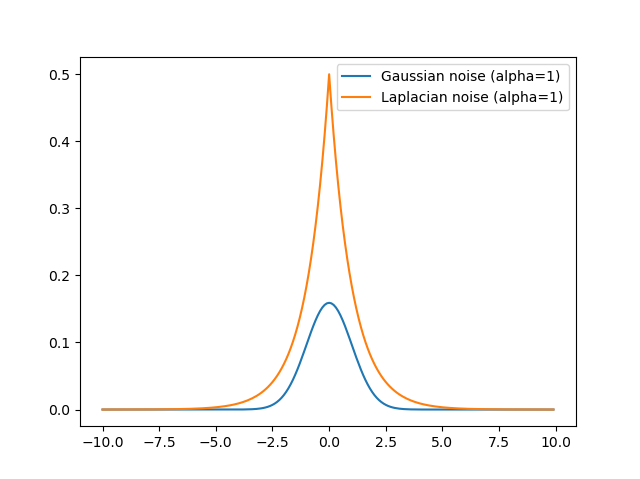
\includegraphics[scale=.3]{C4-1.png}	
	\title{\small{Laplace distribution and Gaussian distribution with $\alpha=1$.}}
	\end{wrapfigure}
	Ridge regression addresses on over-fitting by penalizing the $l_2$-norm of weight vector,
	
	\begin{equation*}
	\min_\mathbf{w} \sum_{i=1}^m (\mathbf{w\phi}_i(\mathbf{x}) - y_i)^2 + \lambda\|\mathbf{w}\|^2_2
	\end{equation*}

	If we assume a Gaussian prior for the weight vector, $\mathbf{w}\sim\mathcal{N}(0,\alpha^{-1}\mathbf{I})$,  the posterior of the training sequence is:
	
	\begin{equation}
	p(\mathbf{w}|S) \propto p(\mathbf{w}) p(S|\mathbf{w}) \propto \exp \left( -\frac{\alpha}{2} \mathbf{w}^\top \mathbf{w} \right) \cdot \prod_{i=1}^N \exp \left( -\frac{(y_i-\mathbf{wx}_i)^2}{2\beta} \right) 
	\end{equation}
	
Maximizing the log posterior function is equivalent to the ridge regression.
	
	
\subsubsection{Lasso}

	Lasso addresses on over-fitting by penalizing the $l_1$-norm of weight vector,
		
	\begin{equation*}
	\min_\mathbf{w} \sum_{i=1}^m (\mathbf{w\phi}_i(\mathbf{x}) - y_i)^2 + \lambda\|\mathbf{w}\|_1
	\end{equation*}
	
	If we assume a Laplace prior for the weight vector, $p(\mathbf{w})=\frac{1}{2\alpha} \exp \left( -\frac{\|\mathbf{w}\|_1}{\alpha} \right)$, then the posterior is:
	
	\begin{equation}
	p(\mathbf{w}|S) \propto p(\mathbf{w}) p(S|\mathbf{w}) \propto \exp \left( -\frac{\|\mathbf{w}\|_1}{\alpha} \right) \cdot \prod_{i=1}^N \exp \left( -\frac{(y_i-\mathbf{wx}_i)^2}{2\beta} \right)
	\end{equation}

Maximizing the log posterior function is equivalent to the Lasso model.

	
	
	\subsection{Predictive distribution}
	
	\subsection{Equivalent kernel}

\end{document}